\documentclass[10pt]{article}
\usepackage{ctex}
\usepackage{graphicx}
\graphicspath{{E:/大学课程/大一下/人工智能程序设计/作业集/第七周作业/图片集/},{pics/}}
\usepackage{amsmath}
\usepackage{amssymb}
\usepackage{float}%使图片紧跟在文字后面

\title{第七周问答作业}
\author{朱士杭\ 231300027}
\date{\kaishu \today}


\begin{document}
	\maketitle
	\section{如何使用函数对功能进行抽象,有什么优势及可能存在的问题?}
	通过一个函数实现某一个功能,当在程序中需要使用该功能的时候,直接调用该函数即可,没有必要再对该功能的代码再写一遍\par
	\subsection{优势}节省代码量、修改的时候比较方便、提高开发效率、层级之间比较分明对于整体程序框架结构更明了
	\subsection{可能存在的问题}可能会产生副作用、函数不灵活对功能抽象的时候需要很多函数的复合相互调用导致程序更加复杂
	\section{对比C/C++以及python对函数嵌套的规定,并简述允许函数嵌套对程序设计的影响}
	\subsection{对比}
	1. C++不允许在函数中定义函数,但是python允许,并且优先调用local-frame中定义的函数\par
	2. C++和python都允许在一个函数中调用另一个函数,并且在栈中创建一个新的相对独立的空间给这个新函数,使得函数之间会有层次感
	3. C++中可以通过函数指针进行传参,python是将函数名对象作为参数进行传递,相似之处在于可以使用传入进来的函数形参,使得函数使用更加灵活\par
	\subsection{影响}
	1. 允许函数嵌套使得程序设计更具有结构化\par
	2. 函数嵌套使得程序员开发的时候将大量的时间可以放在逻辑设计上而不是写大量冗杂的代码\par
	3. 使得程序设计更加灵活,不用总是ctrl-c、ctrl-v复制粘贴大量相似的代码,避免污染眼睛\par
	3. 在Python中,Decorator是什么?请解释装饰器如何工作,以及如何使用它们来修改或增强已有函数的行为。
	\section{请编写一个用于性能检测的装饰器,可以输出被他装饰的函数的运行时间}
	python装饰器是闭包的一种应用,用于拓展原来函数功能的一种函数,这个函数的特殊之处在于它的返回值也是一个函数,
	使用python装饰器的好处就是在不用更改原函数的代码前提下给函数增加新的功能,使用时在需要装饰的函数前一行加上@装饰函数即可
	编写一个用于性能检测的装饰器代码如下:\par
	\begin{figure}[H]
		\centering
		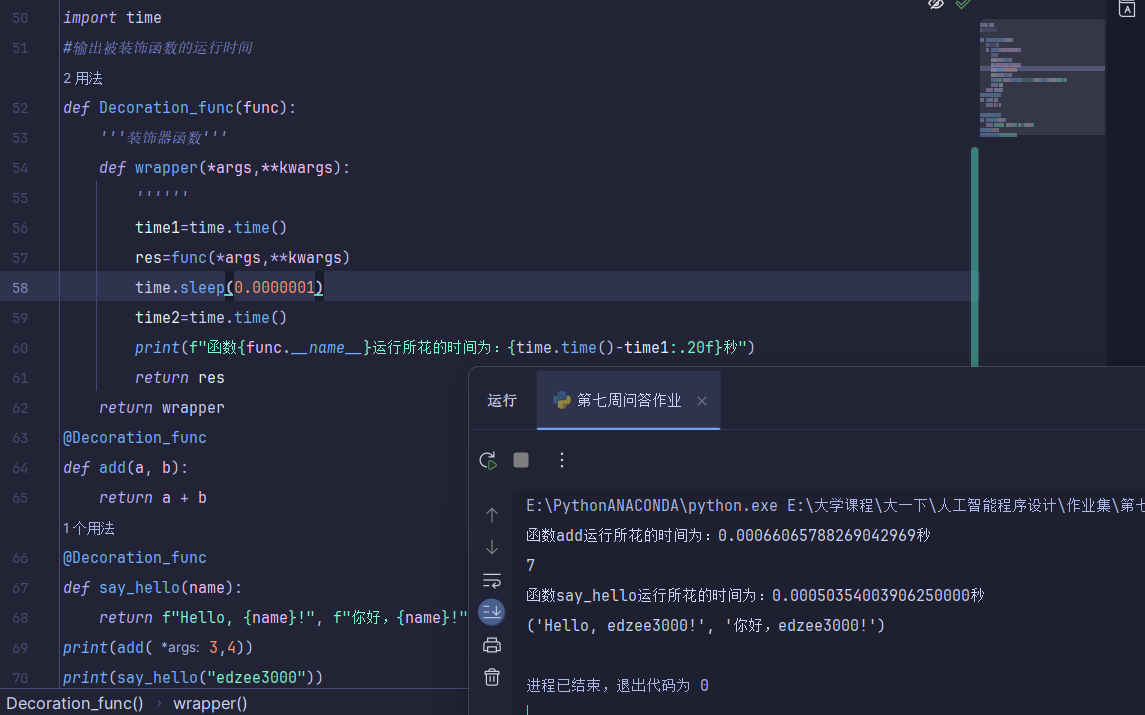
\includegraphics[scale=0.45]{装饰器}
		\caption{自定义装饰器来测试函数性能/运行时间}
	\end{figure}
	\section{折扣策略}
	\subsection{实现每种折扣策略具体的折扣计算函数}
	\begin{figure}[H]
		\centering
		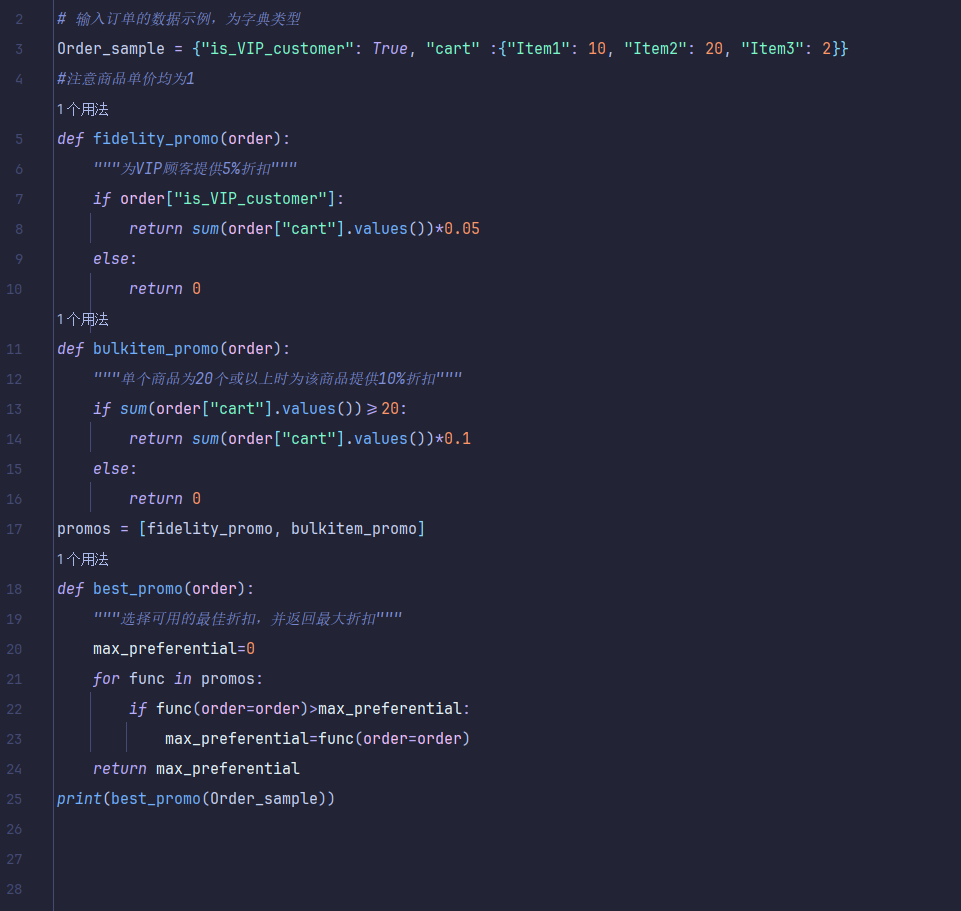
\includegraphics[scale=0.42]{A}
		\caption{折扣计算函数}
	\end{figure}
	\subsection{额外的折扣策略}
	\begin{figure}[H]
		\centering
		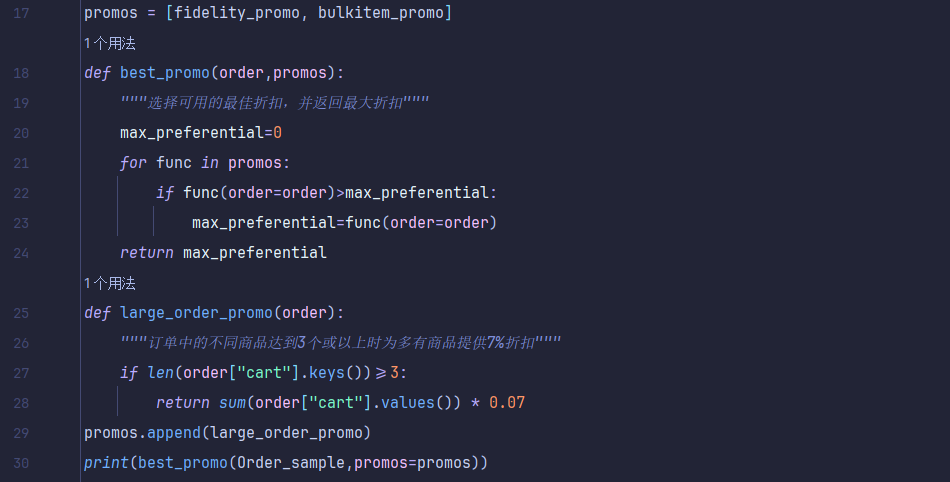
\includegraphics[scale=0.5]{B}
		\caption{额外折扣计算函数}
	\end{figure}
	\subsection{装饰器函数}
	\begin{figure}[H]
		\centering
		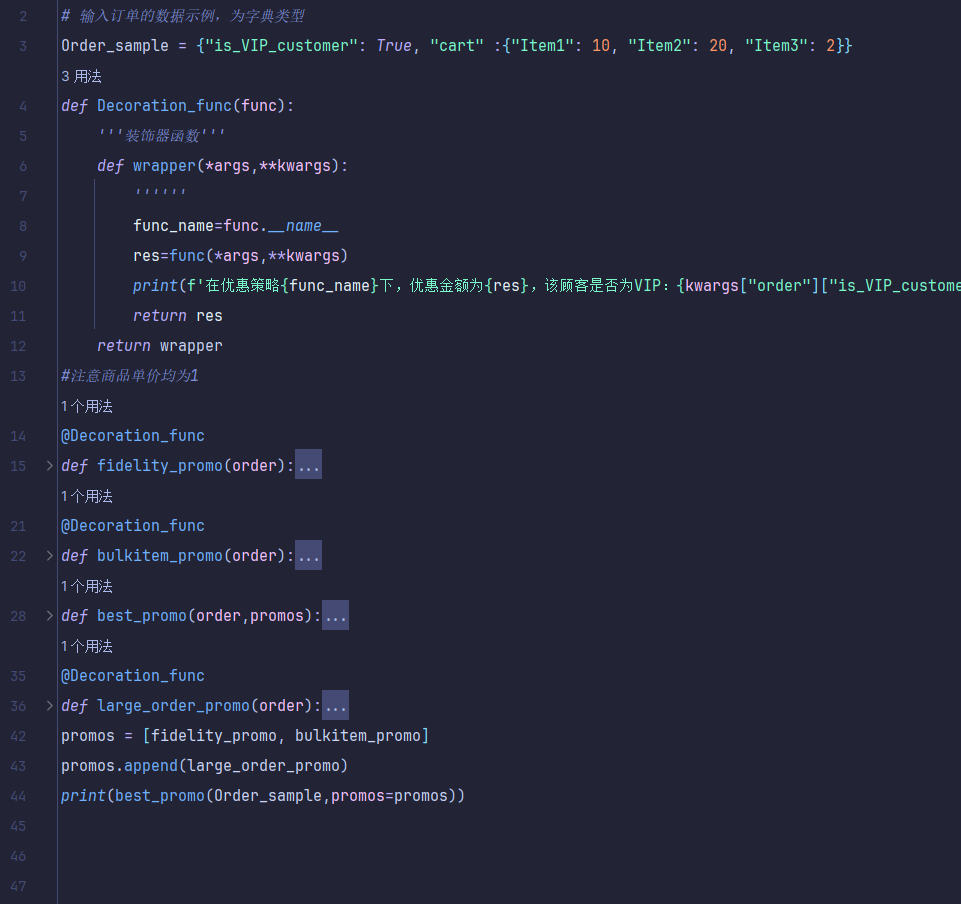
\includegraphics[scale=0.5]{C}
		\caption{装饰器函数}
	\end{figure}
	\subsection{装饰器函数的作用与适用范围}
	\subsubsection{作用}在Python中,装饰器的作用主要是为了增加现有代码(函数、方法或类)的行为,而不需要改变代码本身
	\subsubsection{适用范围}它允许程序员以声明性的方式扩展函数的功能,在日志记录、性能测试、事务处理、缓存、权限校验等方面都是适用的。
\end{document}